\chapter{\textbf{Backround}}
This chapter presents the background knowledge for understanding our work in this thesis. Particularly, Section \ref{sec:NFV} provides a summary of basic knowledge on NFV architecture. Section \ref{sec: MEC} gives an introduction of the newly emerged MEC technologies. Section \ref{sec: SFC} specifically focus on the SFC architecture and its optimization opportunities. Then, Section \ref{sec:online learning} discusses the online learning techniques and especially the \ccmab algorithm adopted in this work in order to solve the user-managed online SFC orchestration problem. Section \ref{sec:mathematical tools} discusses the mathematical techniques employed in this work to model and solve the offline SFC orchestration on edge. Lastly, Section \ref{sec:software tools} gives an overview of the software tools used for simulation and emulation experiments.


\section{Network Function Virtualization}
\label{sec:NFV}
\subsection{NFV architecture}
Network Function Virtualization (NFV) is a network architecture concept that is first introduced in 2012 by the European Telecommunications Standards Institute (ETSI) \cite{nfv_wp}, in which they propose to softwarize the traditional network appliances that are physically installed (\eg, Deep Packet Inspection (DPI), Firewall, Message Router), and implement these functions in a way that they can be run on a range of industry-standard server, and can be migrated and placed in various locations in the network as required, without the need of installing new physical equipment. Each softwarized implementations of these network appliances are defined as a virtual network function (VNF). These VNFs can be automatically and remotely installed in a shared computing platform and have functionality as their hardware counterparts in principle.
An example of the NFV paradigm is shown in fig \ref{fig:NFVenvironment}, where  specialized middleboxes are replaced with VNFs consolidated on Commodity Off-The-Shelf (COTS) hardware \cite{zhang2020nfv}.
\begin{figure}
	\centering
	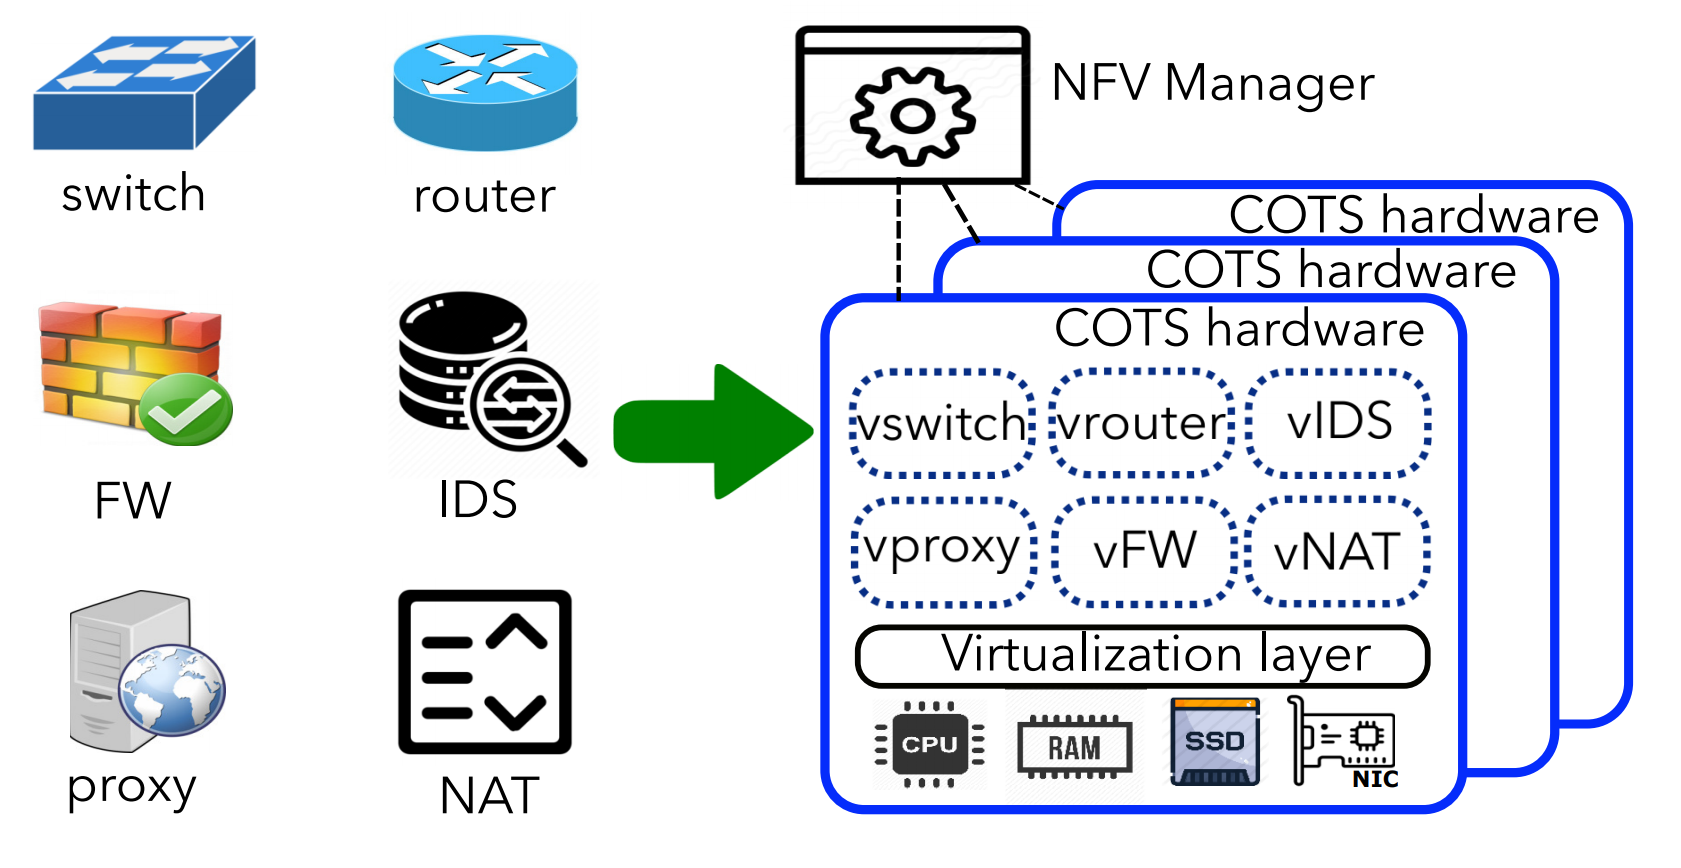
\includegraphics[width=0.9\linewidth]{figs/NFVenvironment.PNG}
		\vspace{\baselineskip}
	\caption{An illustrative example of NFV paradigm \cite{zhang2020nfv}}
	\label{fig:NFVenvironment}
\end{figure}
Virtualising Network Function has potential benefits such as reducing equipment cost, increasing the speed of Time to Market (\ie, the time it takes to implement a network service), and enabling multi-tenancy/multi-version network appliances. Moreover, NFV architecture provides users with enhanced manageability over their personalized applications. 
Compared to traditional network architectures, the advantages of adopting NFV can be summarized according to NFV white paper~\cite{nfv_wp} as follow:
(1) reduced equipment costs, 
(2) improved operating performance and operational efficiency,
(3) optimized network configuration and resource allocation,
(4) flexible network function deployment and dynamic operation, and (5) reduced energy consumption.

\subsection{NFV optimization}
Furthermore, NFV architecture provides various optimization opportunities for researchers such as latency, resource consumption, VNF deployment cost minimization, and utility maximization. In a typical resource allocation problem in an NFV-based network (NFV-RA), there are three stages described below.

1) \textit{VNF chain composition}: VNF chain composition, referred to as Service function Chaining in this work, is the problem of dynamically and strategically composing and deploying SFCs on a set of physical works in an NFV architecture, in order to meet a predefined service requirement. 
%The first challenge is the chaining of the VNFs to implement a requested network service.
%Figure \ref{fig:SFCcomposition} shows an example of two possible chainings of a Virtual Network Functions Request (VNFR), in which the SFC starts from VNF1 and terminates at VNF5, In VNF-FG2,
%the VNF composition is different as the VNF4 precedes VNF3 in the lower branch, which can be another feasible solution.
%\begin{figure}
%	\centering
%	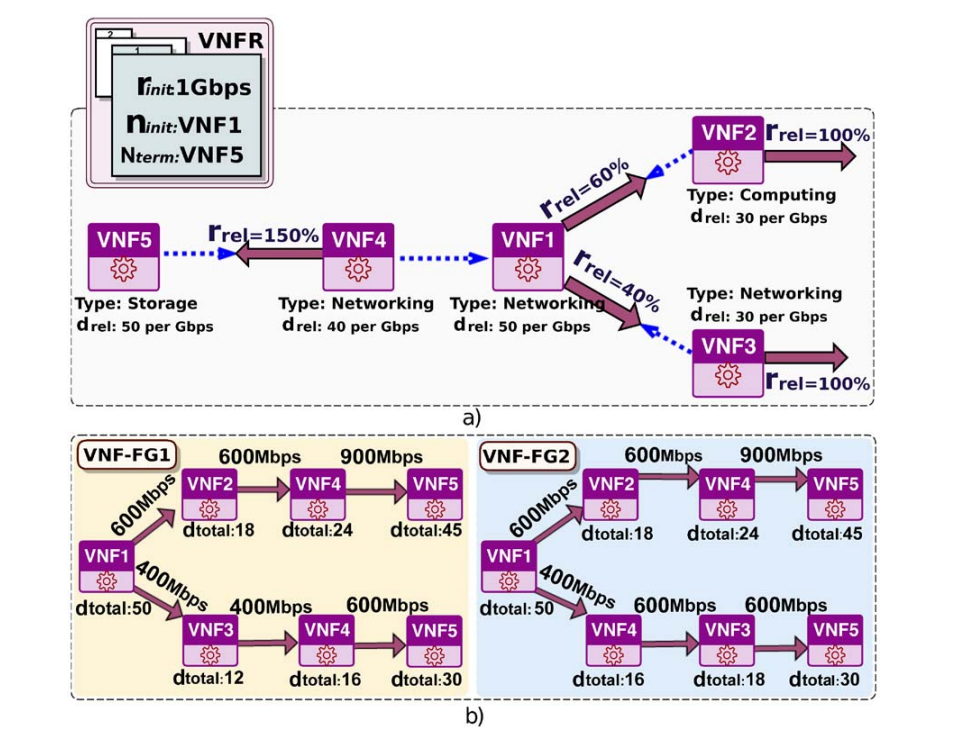
\includegraphics[width=0.9\textwidth]{figs/SFCcomposition.PNG}
%		\vspace{\baselineskip}
%	\caption{VNF Chain composition \cite{herrera2016resource}}
%	\label{fig:SFCcomposition}
%\end{figure}


2) \textit{VNF Chain Embedding}: The second stage is called VNF Chain Embedding, also referred to as SFC placement or orchestration in this work, which aims to find the physical node in the network infrastructure to employ the VNFs that suits the requested network services. Figure \ref{fig:SFC embedding} shows an example of an end-to-end VNF chain (Firewall $\rightarrow$ LoadBalancing $\rightarrow$ Encryption $\rightarrow$ PacketInspection $\rightarrow$ Decryption) embedding.


\begin{figure}
	\centering
	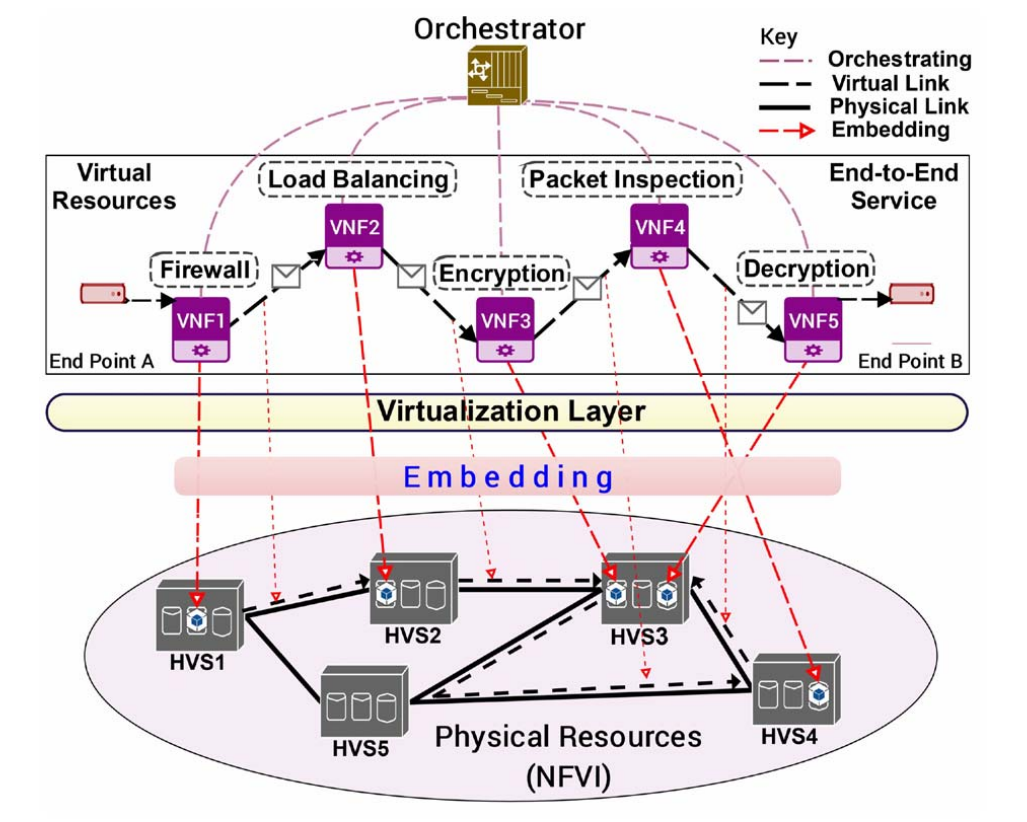
\includegraphics[width=0.9\linewidth]{figs/SFCembedding.PNG}
		\vspace{\baselineskip}
	\caption{VNF Chain Embedding \cite{herrera2016resource}}
	\label{fig:SFC embedding}
\end{figure}

3) \textit{VNF Chain Scheduling}: The final stage is to schedule the VNFs on the chain properly. Specifically, this stage seeks to minimize the total execution time of the requested network services by scheduling the execution of each VNF, for example, execute some VNFs simultaneously or execute each VNF in order of the chain. 
%Figure \ref{fig: VNF Chain Scheduling} showing an example of how the same VNF chain can be scheduled in three different ways.
%\begin{figure}
%	\centering
%	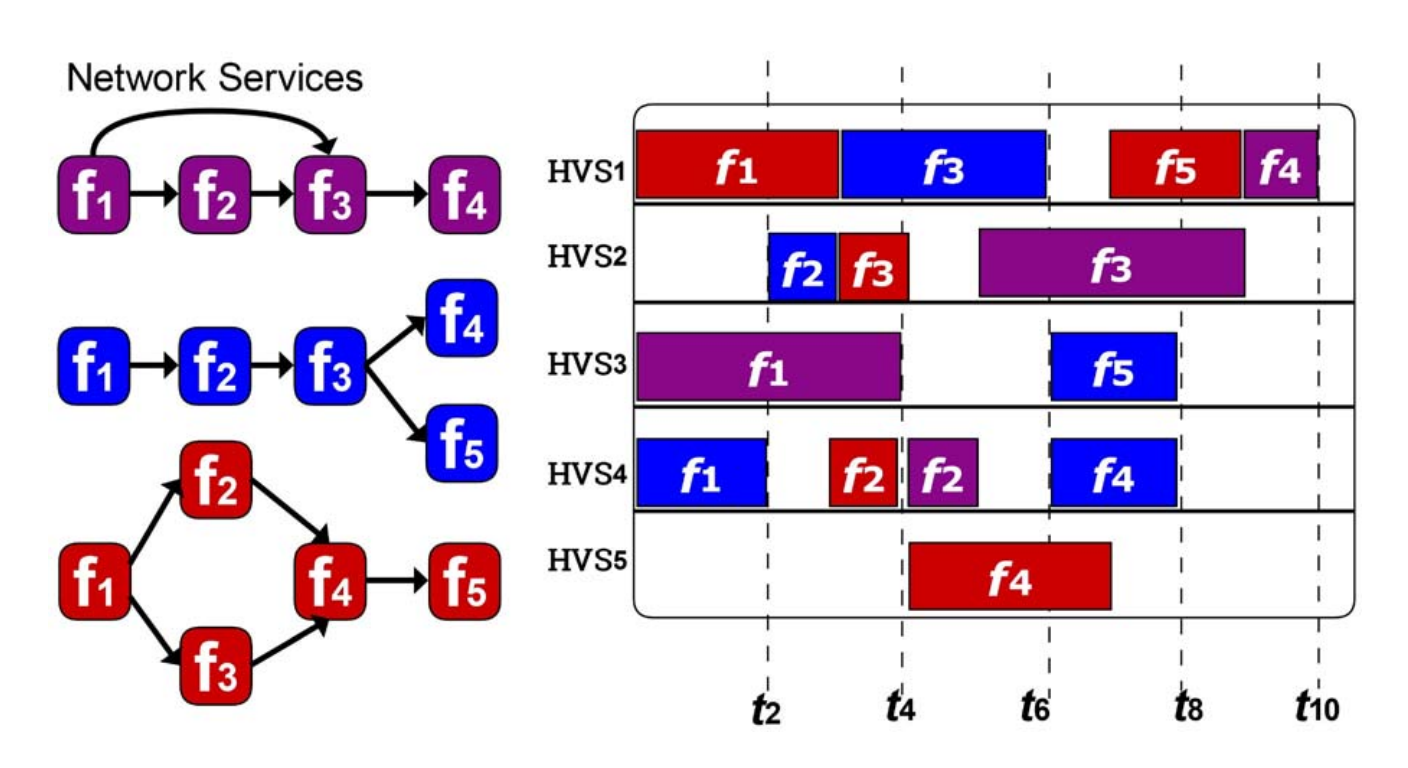
\includegraphics[width=0.9\linewidth]{figs/VNFSchedule.PNG}
%		\vspace{\baselineskip}
%	\caption{VNF Chain Scheduling \cite{herrera2016resource}}
%	\label{fig: VNF Chain Scheduling}
%\end{figure}


In this work, our focus is mainly on the second stage of an NFV-RA problem, that is, the placement/embedding/orchestration of the VNF chain to physical, we refer to it as \textbf{SFC orchestration} in this thesis. In section \ref{sec: SFC} we further discuss the standard SFC architecture,  mathematical and algorithmic approaches for SFC orchestration.






%The work in this thesis concerns the minimization of end-to-end delay while taking resource consumption into consideration. 

\section{Mobile Edge Computing}
\label{sec: MEC}
\subsection{MEC architecture}
Mobile Edge Computing (MEC) was first standardized by European Telecommunications Standards Institute (ETSI) and Industry Specification Group (ISG), it is introduced as an integration of edge computing (also known as fog computing) and mobile computing, which empowers Mobile Cloud Computing (MCC) by distributing cloud resources (\eg storage and processing capacity) to the edge servers inside the range of radio access network (RAN). 
An illustration of a MEC system is shown in fig \ref{fig:MECachitecture}, which consists of two major components: mobile devices (e.g. end-users, clients, and service subscribers) and MEC servers. MEC server is usually
a small data center deployed by cloud and telecom operators that can be placed close to the end-user and co-located with the wireless APs. The edge servers are connected to the data centers through a gateway via a backbone internet, while mobile devices are connected to the edge servers via a well-established wireless link implemented using advanced wireless communications and network technologies \cite{MECsurvey}.
%
In section \ref{section: system model} we present our system model formulation for MEC that consist of one cloud center and multiple edge servers.
%
\begin{figure}
	\centering
	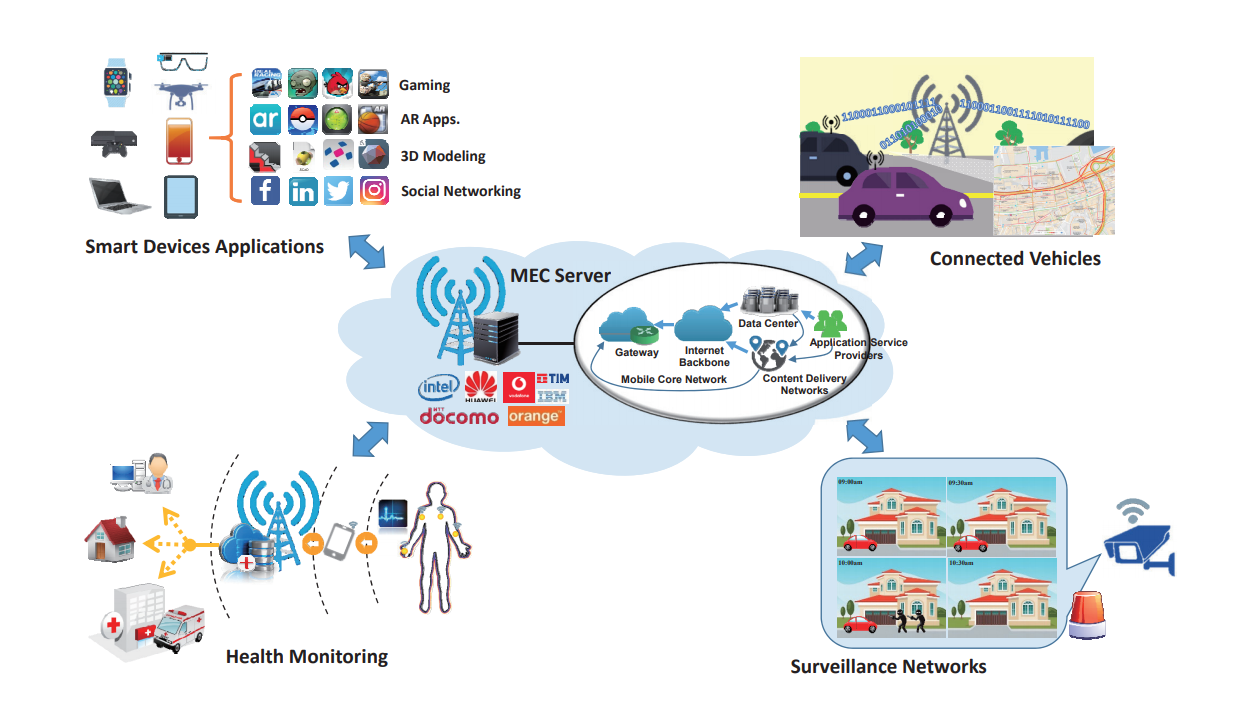
\includegraphics[width=0.9\linewidth]{figs/MEC architecture.PNG}
		\vspace{\baselineskip}
	\caption{Architecture of the MEC system \cite{MECsurvey}}
	\label{fig:MECachitecture}
\end{figure}

Numerous works in different fields have been discussed in the literature that can be exemplified as a application scenario for MEC, including but not limited to: Health care \cite{apphealthcare1}, Video Analytics\cite{appvideoanalytics1}, Mobile Big Data Analytics \cite{appmobilebigdata1}, Connected Vehicles \cite{appconnectedvehicles1}, Smart Grid\cite{appsmartgrid1}, Wireless Sensor and Actuator Networks \cite{appwsn1}, Smart building Control, SDNs \cite{appsdn1}, Ocean Monitoring \cite{appoceanmonotoring1}. According to the white paper published by ETSI \cite{MECwhitepaper}, a brief summary of the key features of MEC is characterized below.

\cat{On-premises} MEC can run isolated from the rest of the network while having access to local resources. This plays an essential role in Machine-to-Machine (M2M) scenarios such as security or safety systems that require high-level resilience.

\cat{Proximity} Being close proximity to resources, MEC has an advantage in capturing and analyzing big data. It also provides direct access to devices, which can benefit compute-hungry applications such as augmented reality (AR) and video analytics.

\cat{Lower Latency} Edge server is usually deployed at the nearest location of the mobile user, which considerably reduces user-perceived latency to their devices. This can greatly boost user experience and reduce the congestion of other parts of the network.

\cat{Location awareness}  MEC devices can utilize low-level signaling information to determine the location of other connected devices under different types of the wireless network, which provide mobile users with location-based services and analytics.

\cat{Network context awareness} RAN Real-time network information such as the congestion of the radio cell and network bandwidth can be estimated by applications that adopt MEC in their implementation. This offers context awareness that can help to improve the mobile user's experience.

In summary, MEC provides the end-user with swift and powerful computing, energy efficiency, storage capacity, mobility, location, and context awareness support. 
%

\subsection{MEC research topics}
MEC has provided numerous research topics in computer science, and we summarize the main topics that have been studied in this area and discuss where our work stands.

\cat{Computational Offloading}
The most discussed research topic in the MEC area is computation offloading, which is the process of migrating computing tasks to external resources such as clouds, grids, or clusters \cite{ma2013mobile}.
This increases the computing ability of mobile devices by running computing-intensive and resource-demanding applications (e.g. 3-D gaming and video encoding) on edge cloud. 
For example, offloading web application execution on the edge servers that is within the RAN can accelerate web browsing \cite{takahashi2015analysis}.

Using well-designed algorithms and approaches, the computational offloading process can also be optimized in a radio access environment, which can reduce signal interference and energy consumption \cite{chen2015efficient, sardellitti2015joint}. 



\cat{Low Latency}
MEC can greatly improve users' experience by lowering the latency of their requested applications and services. 
For example, latency can be effectively reduced by intelligently scheduling memory replication events in the edge cloud while resolving conflicts for wireless resources\cite{abdelwahab2015replisom}.
%
Integrated with 5G technologies, MEC can provide real-time context-aware support for applications such as live remote robotic telesurgery and road accident\cite{nunna2015enabling}, which require context-information (e.g. geographical information). MEC allows ultralow latency for these applications by satisfying the context demands.
%
MEC can also support vehicular delay-tolerant network by utilizing smart grid devices that communicate with the MEC environment. It addresses the communication complications caused by the high mobility of vehicles by interacting with mobile smart devices that monitor the data sets\cite{kumar2016vehicular}.

\cat{Storage support}
MEC also provides users with additional storage support when their local device storage is limited. MEC storage capabilities can be further enhanced by integrating with virtualization techniques such as software-defined network, software-defined compute, and software-defined storage\cite{jararweh2016sdmec}, which enable the support for storage/computing-intensive applications such as traffic monitoring and mobile gaming.

\cat{Energy Efficiency}
By running computational tasks on edge cloud architecture, MEC can reduce the energy consumption of users' local devices. 

For example, mobile devices can share the energy and computational resources on edge by adequately estimating the network status, which ensures the computation time is synchronized \cite{gao2014opportunistic}. 
%
MEC can significantly prolong the battery lifetime of user devices by offloading computing-intensive tasks like video encoding to the edge servers that employ advanced encoding services\cite{beck2015me}. Instead of migrating computing-intensive to the edge, MEC architecture can also coordinate resources between resource-rich mobiles devices and resource-constraint mobile devices in order to escalate the power management of these devices.

In this work, our focus is on computational offloading and latency reduction in MEC architecture. In particular, we consider the optimization of the end-to-end latency to run SFCs in MEC, for which we design an online SFC orchestration algorithm and offload SFC tasks accordingly.







\section{Service Function Chain}
\label{sec: SFC}
Service Function Chain is defined as a sequence of multiple VNFs that user's traffic has to traverse through to realize their required services. This section provides some background knowledge of SFC, including SFC architecture, SFC request model,  SFC Resource allocation problems, and optimization approaches.
\subsection{SFC architecture}
A typical SDN-based SFC architecture consists of the SFC control plane and  SFC data plane, as defined by the IETF SFC and ONF working groups. Fig \ref{fig:SFCachitecture} shows an illustration of a standard SFC architecture that is explained as follows:

\cat{SFC control plane} The control plane is responsible for the management of SFC, such as the management of each service function instance (SFI), the mapping of SFC to a specific service function path (SFP), the administration of forwarding rules, and the adjusting of SFP with regards to the link status.

\cat{SFC data plane} SFC data plane consist of: SFC classifier, Service function forwarding (SFF), Service function (SF) and SFC proxy. the SFC classifier differentiates the incoming traffic into flows and tags each flow with an SFP header. An SF executes a particular set of actions on the incoming packets (e.g deep packet inspection or firewall functions). An SFC proxy de-capsulate the packets when the majority of SFs do not recognize the SFC packet headers.
\begin{figure}
	\centering
	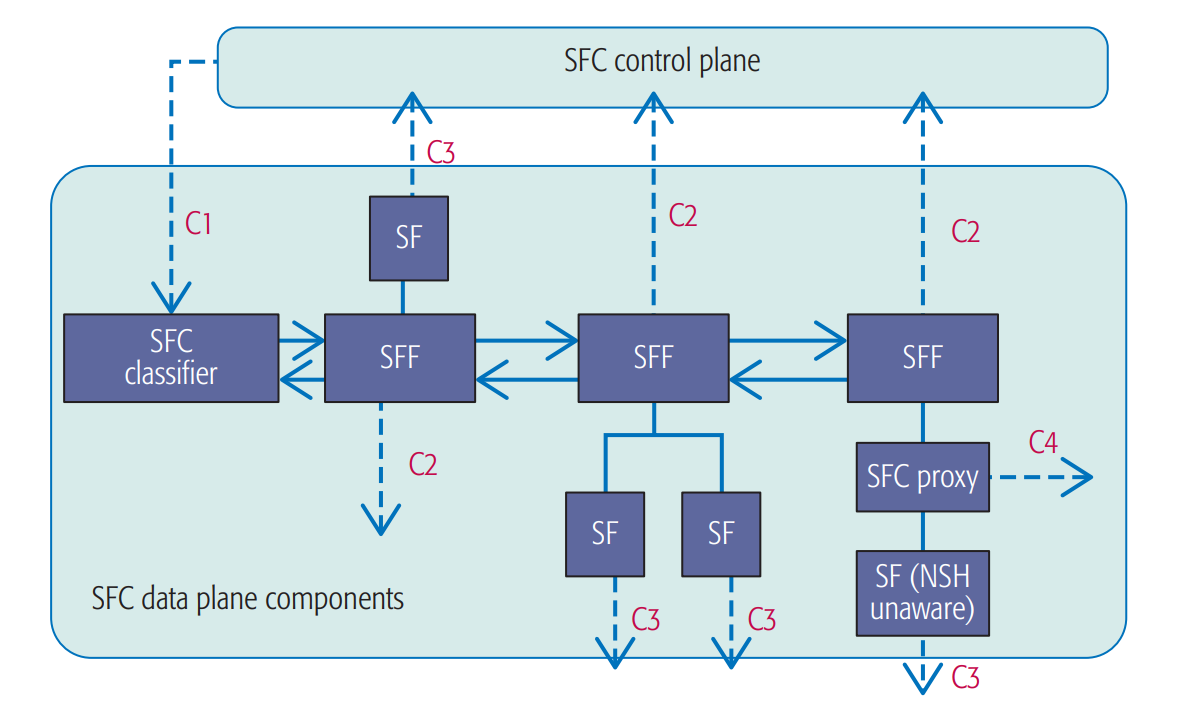
\includegraphics[width=0.9\linewidth]{figs/SFCarchitecture.PNG}
		\vspace{\baselineskip}
	\caption{A typical SFC architecture \cite{medhat2016service}}
	\label{fig:SFCachitecture}
\end{figure}

\subsection{SFC request model}
In order to realize a particular service, the user's traffic flow must be directed through an ordered sequence of VNF instances. For example, an SFC of NAT, FW, and IDS, as depicted in fig \ref{fig:SFCrequestmodel}. The set of enabled services represents the operators'
services, which is built according to the service agreements between
operators and end-users with regards to network policies \cite{xie2016service}

An SFC request is a source-to-destination path that contains an ordered list of service functions, and the users may have various bandwidth and computational demands for each service function. We model our SFC demand in section \ref{sec:SFCrequest}, in which we define $\lambda$ as the user-generated traffic rate and add customized scale factor $\alpha_{s_i}$ to it with respect to each type of service $s_i$.

\begin{figure}
	\centering
	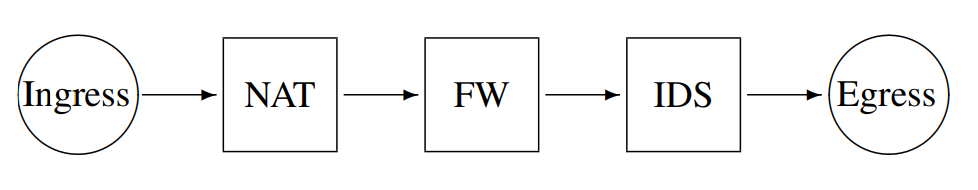
\includegraphics[width=0.9\linewidth]{figs/SFCrequestmodel.PNG}
		\vspace{\baselineskip}
	\caption{Service Request Model \cite{xie2016service}}
	\label{fig:SFCrequestmodel}
\end{figure}

\subsection{SFC orchestration problem}

\cat{Delay Aware} In a delay-aware SFC orchestration problem, a physical network and a set of service requests are given, as well as the number of needed VNF types and demand specifications. The goal is to minimize the total end-to-end delay. Therefore delay-aware SFC orchestration problem has two steps:

\begin{enumerate}
	\item Calculate the latency on each link and node with regards to the service demand and capacity.
	\item Place SFCs to physical nodes and links such the total end-to-end delay is minimized.
\end{enumerate}

\noindent In addition, a virtual link on SFC may be placed on several physical links.

\cat{Cost Aware} The objective of the cost-aware SFC orchestration problem is to minimize the deployment cost when placing SFCs to physical nodes and links, which is often expressed as the resource and bandwidth consumption.








\subsection{SFC orchestration optimization approaches}
To orchestrate a SFC via an NFV architecture, the user needs to choose a set of computing platforms to install each VNF on a SFC and decide the SFC's routing order while considering various constraints such as fluctuated SFC demands and quality of service (QoS). The problem of SFC orchestration is one of the main challenges in NFV. Therefore many works have taken aims at addressing it, and many optimization approaches have been investigated. They can be summarized as below.

\cat{Exact and approximation solutions} SFC orchestration problem can be typically formulated into: Integer Linear Programming (ILP) or Mixed Integer Linear Programming (MILP). We can use traditional exact approaches to solve ILP, \eg, \textit{dynamic programming, branch and bound, cutting plane methods}
The work in this thesis uses DP to solve per-time-slot SFC orchestration in a guaranteed time. \textit{Approximation solutions} give a trade-off between optimal solution and algorithm complexity, which achieves a near-optimal but polynomial-time performance.

\cat{Heuristic solutions}
In practice, SFC orchestration is required to be low latency or real-time. Thus fast heuristics-solution is often preferred due to the hardness of the SFC orchestration problem. \eg, \textit{simulated annealing, tabu search, genetic algorithm, ant colony, best-fit decreasing}. 


\section{Learning algorithm}
In this section, we discuss the learning algorithms we applied in this work.
\label{sec:online learning}
\subsection{Online learning}
Online learning is the process of taking actions given knowledge of rewards of the previous actions and possibly available information. It takes place in continuous rounds. On each round, the learner is presented with a set of actions and is required to take one of them. The goal of online learning is to maximize the accuracy of the learner's predictions so that correct decisions can be made, which is in contrast to a traditional offline learning method that is to learn a model from the entire training data set at once \cite{hoi2018online}. 
Therefore, online learning can instantly learn from newly arrived data and are easier to implement than offline learning. In this work, user-managed SFC orchestration can be modeled as an online learning process due to the sequentialness of the user requests.

Online binary learning can be exemplified as a simple online learning, where the reward/outcome of each action is binary: yes or no.  Algorithm \ref{alg:online binary learning} summarizes a brief procedure of online binary learning, where $\nb{x}_t$ denotes the sequential instance and $y_t$ denotes the binary reward label of each instance. At each round, the learning use vector $\nb{w}_t$ as a prediction model to calculate the predicted reward label : $\hat{y}_t = \textnormal{sign}( \textbf{w}_t^\top \textbf{x}_t)$. Then the learner receives the true reward label $y_t$ after taking the predicted action, and calculate the suffered loss: $l_t(\textbf{w}_t) = \textnormal{max}(0,1-y_t\textbf{w}_t)^\top \textbf{x}_t)$. Lastly, the learner strategically update the prediction model based on the loss and true labels received. 
\begin{algorithm}
	\caption{Online Binary Learning}
	\label{alg:online binary learning}
	Initialize the prediction function as \textbf{w_1};\\
	\For{$t=1,2,...,T$}{
		\textnormal{Receive instance: $\nb{x}_t \in \mathbb {R}^d;$}\\
		\textnormal{Predict $\hat{y}_t = \textnormal{sign}( \textbf{w}_t^\top \textbf{x}_t);$} \\
		\textnormal{Receive the true reward label: $y_t \in \{ -1, +1\};$}\\
		\textnormal{Suffer loss: $l_t(\textbf{w}_t) = \textnormal{max}(0,1-y_t\textbf{w}_t)^\top \textbf{x}_t);$}\\
		\textnormal{Update the prediction model} $\textbf{w}_t$ to $\textbf{w}_{t+1};$
	}
	\textnormal{Calculate regret:} $R_T = \sum^T_{t=1} l_t({\bf w_t}) - \min _{\bf w} \sum_{t=1}^T l_t({\bf w});$
\end{algorithm}





\subsection{Bandit online learning}
As an import branch of online learning, Bandit online learning, a.k.a. Multi-Armed Bandit (MAB) problem, has been studied extensively in the online learning community.
MAB is normally formulated as a sequential decision-making problem where the decision-maker is presented with $m$ arms to select from at each of $n$ rounds, where $T$ is often unknown at the beginning and decisions are made based only on the feedback from the environment. The distribution of reward on each arm is unknown, and the goal of the problem is to maximize the total reward or minimize the total loss over the course of $n$ rounds, with $a_t$ denoting the action of each round, $r_t(a_t)$ and $l_t(a_t)$ denoting the reward and loss of that action respectively. We can formally define the "regret" as the difference of cumulative loss between the optimal arms and player selected arms:
\begin{equation}
	R_T = \sum\limits_{t=1}^T l_t(a_t) - \min\limits_{i\in[m]} \sum\limits_{t=1}^T l_t(i)
\end{equation}
One of the major challenges of MAB is how to trade-off between \textit{exploitation} and \textit{exploration}, where \textit{exploitation} of past actions ensure high payoffs based on the past knowledge and \textit{exploration} of new actions gives possibly higher payoffs in the future, which is also one of the major concerns in this work.


\cat{$\epsilon$-Greedy Multi-Arm Bandit}
The first simplest MAB based algorithm is $\epsilon$-Greedy MAB introduced in \cite{sutton1998introduction}, in which the player plays the arm that currently has the highest average reward with probability $1-\epsilon$ and plays a random arm with probability $\epsilon$, where $\epsilon$ is a constant value in (0, 1). $\epsilon$-Greedy Multi-Arm Bandit algorithm is summarized in algorithm \ref{alg:greedymab}, where $N_{i_t}(t)$ denote the number of times arm $i$ has been selected by the player until $t$ rounds and $\mu_{i_t}$ denotes the mean of the rewards received on arm $i$. 

In this work, $\epsilon$-Greedy Multi-Arm Bandit algorithm is used as a performance comparison in experiments presented in chapter \ref{chapter:simulation} and \ref{chapter: Mininet-wifi Experiments}. 

\begin{algorithm}
	\caption{$\epsilon$-greedy MAB}
	\label{alg:greedymab}
	\textbf{INPUT:} parameter $\epsilon > 0$\\
	\textbf{INIT:} empirical means $\mu_i = 0, \forall i \in [m]$\\
	\For{$t=1, 2, ..., T$}{
		with probability 1-$\epsilon$ play the current best arm $i_t = \textnormal{argmin}_{i\in[m]}\mu_i$\\
		with probability $\epsilon$ play a random arm\\
		receive $l_t(i_t)$ and $r_t(i_t)$\\
		update the empirical means $\mu_{i_t} = (\mu_{i_t}*N_{i_t}(t) + r_t(i_t))/(N_{i_t} + 1)$\\
	}
	
	
\end{algorithm}







\cat{Contextual Combinatorial Multi-Arm Bandit}
In the framework of a Combinatorial multi-armed bandit (CMAB), the decision-maker needs to select a set of arms(referred to as a super arm) and play it,  after a super arm is played and the reward of each arm in the super arm and other triggered arms are revealed at each round. When each arm can be characterized by a feature vector that the decision-maker is able to observe, the problem is known as Contextual Combinatorial Multi-arm bandit (\ccmab) problem, which is often used to adapt to user feedback and diverse interest.
Our work is inspired by the contextual combinatorial upper confidence bound algorithm (\ccucb) presented in \cite{ccmab}, which is a general algorithms for addressing \ccmab problems. \ccucb\ characterize the user-observed context using a set of
feature vectors $\textbf{X}_t = \{\textbf{x}_t(i), ..., \textbf{x}_t(m)\}$ corresponding to $m$ arms at each round $t$ and use vector $\theta_*$ to characterize the system feature, which is unknown to user. 
\ccucb\ then define the reward function on each arm to be:
\begin{equation}
	\label{eqn:computesore}
	r_t(i) = \theta_*^T\textbf{x}_t(i) + \epsilon_t(i),
\end{equation}
where, $\epsilon_t(i)$ is a zero-mean random variable that represent the noise in the system. The goal of \ccucb\ is to maximize the expected cumulative reward $\E [\sum_{t\in n}R_t(S_t)]$ over n rounds, where $R_t(S_t)$ represent the sum reward received for all the arms on the selected super arm $S_t$ at round $t$.
The algorithm use the feature vectors and previously observed rewards to maintain a confidence set for true parameter $\theta_*$, which is then used to compute an reward upper confidence bound for each arm:
$ \hat{\textbf{r}}_t = {\hat{r}_t(1), ..., \hat{r}_t(m)} $
according to equation \ref{eqn:computesore}. $\hat{\textbf{r}}_t$ and $\textbf{X}_t$ is taken as a input to a computation oracle that computes the optimal or near-optimal super arm $S_t$. The algorithm plays the returned super arm and update the confidence sets using the observed rewards on the super arm.
The pseudocode of \ccucb\ is summarized in algorithm \ref{alg:ccucb}, 
where $\alpha_t$ is an approximation ratio that shows the proximity of the current solution to the optimal solution, $\textbf{V}_t$ and $\textbf{b}_t$ are two auxiliary vectors used to update the system paramter $\theta_t$.

In this work, chapter~\ref{chapter: Proposed Method} presents our proposed algorithm that adopts the \ccucb\ framework, which uses an optimal oracle that is based on dynamic programming (e.g, $\alpha_t = 1$)

\begin{algorithm}
	\caption{\ccucb}
	\label{alg:ccucb}
	\textbf{Input:} \alpha_1, ..., \alpha_n\\
	Initialize \textbf{V}_0 \leftarrow \textbf{I}_{d\times d}, \textbf{b}_0 \leftarrow \textbf{0}_d \\
	\For{t \leftarrow 1, ..., n}
	{
		$\hat{\theta}_t$ \leftarrow \nb{V}^{-1}_{t-1}\nb{b}_{t-1}\\
		\For{i \leftarrow 1, ..., m}{
			$\bar{r}_t(i)$ \leftarrow \hat{\theta}_t^T \textnormal{\bf x}_t(i)\\
			$\hat{r}_t(i)$ \leftarrow \bar{r}_t(i) + $\alpha_t\sqrt{\textnormal{\bf x}_t(i)^T \nb{V}_t^{-1}\textnormal{\bf x}_t(i)}$
		}
		\textbf{S}_t \leftarrow \mc{O}({\hat{\textbf{r}_t}}, \textnormal{\bf X}_t)\\
		\textnormal{Play super arm }\textbf{S}_t \textnormal { and observe} \{r_t(i)\}_{i\in S_t}\\
		\nb{V}_t \leftarrow $\nb{V}_{t-1}$ + \sum_{i\in S_t}\nb{x}_t(i)\nb{x}_t(i)^T\\
		\nb{b}_t \leftarrow \nb{b}_{t-1} + \sum_{i\in S_t} r_t(i)\nb{x}_t(i)\\
	}
\end{algorithm}



\section{Mathematical Tools}
\label{sec:mathematical tools}
In this section, we present the two mathematical tools we used for the optimizations considered in this work.
\subsection{Integer Linear problem}
Integer Linear problem is a type of constrained optimization, which consists of an objective function and a set of constraints. In ILP, all the variables in the objective function are restricted to be integers while all the functions and constraints are linear. In this work, we formulate \myproblem\ as a specific form of ILP that is Binary integer linear problem (BILP), in which all of the variables are binary, that is, they can only take on the value of 0 or 1. This  is often used to represent a selection or rejection of an option, \eg\ a yes/no answer, a turning on/off of a switch, and in our work, a decision of whether or not to select a certain node and link.
Formulation \ref{ILP} illustrates an example of a standard constrained binary integer linear problem. In this program, $x_i$ are the \textit{variables} while $c_i$ and $a_{i,j}$ are the \textit{constant coefficient},  the expression \ref{ILP:objective} describes the objective of the BILP as a linear function of variable $x_i$, expression \ref{ILP:const1} and \ref{ILP:const2} are the inequality and equality constraints that $x_i$ is subjected to respectively , while expression \ref{ILP:const3} restrict $x_i$ to be variables only. An standard form also restricts that the variables are ordered according to the objective function coefficients, which is expressed in constraint \ref{ILP:const4}.
\begin{problemenv}
	\caption{A Standard Binary Integer Linear Program}
	\begin{subequations}
		\label{ILP}
		\begin{align}
			\label{ILP:objective}
			\textbf{ Minimize Z =}  & \sum_{i=1}^nc_ix_i\\
			\label{ILP:const1}
			\textbf{Subject to:}  &\sum_{j=1}^n a_{ij}x_j \leq b_i, \quad\forall i \in {1, 2,    ..., h}\\
			\label{ILP:const2}
			&\sum_{j=1}a_{ij}x_j = b_i, \quad\forall i \in {h+1, h+2, ..., m} \\
			\label{ILP:const3}
			& x_i =  0\ \text{or}\ 1,\quad \forall \in {1, 2, ..., n}\\
			\label{ILP:const4}
			& 0\leq c_1\leq c_2 \leq ...\leq c_n 
		\end{align}
	\end{subequations}
\end{problemenv}

The formulation above may seem restrictive, but it is easy to convert many problems to this form. For example, we can handle the negative objective function by simply replacing $x_i$ with $1-x_i$. Negative constraints can also be handled by converting $\leq$ form to $\geq$ form, and reordering the variables is easy.

\cat{Linearization}
A common linearization of BILP is to linearize a product of multiple binary variables, which can be done by a general method showed in formulation \ref{BILP:linearization}, 
where a product of $n$ binary varibles $x_i$ can be represented by a new binary variable $z$ and additional constraints. The linearization concerned in this work is a product of two binary variables, more specifically, we linearize the migration delay part of the objective using this method as expressed in equation \ref{eqn:objlinearization}.
\begin{problemenv}
	\caption{BIP Product Linearization}
	\label{BILP:linearization}
	\begin{equation}
		\begin{align}
			&z = \prod_{i=1}^n x_i\\
			&z \leq x_i\\
			&z \geq x_i-(n-1)
		\end{align}
	\end{equation}
\end{problemenv}


\subsection{Dynamic program}
A recursive algorithm can be designed to solve the problem more efficiently by taking advantage of the similarities in the substructures of a
problem,\cite{IntroductiontoAlgorithm}.
This type of algorithm first divides the problem into many subproblems recursively, each of which has the same structure. The algorithm then repeatedly calls itself to solve each subproblem. Because the problem is divided recursively, there are many instances where subproblems in different branches of the recursion tree are exactly identical to one another.
Rather than separately solving all subproblems,
which wastes computing resources and time, Dynamic Programming proposes to store the results of the subproblems and reuse them when necessary \cite{IntroductiontoAlgorithm}. By apply such a simple technique,
the number of recursive steps needs to solve the problem can be reduced from exponential to polynomial. DP is an optimization approach that has been widely used in common problems such as Min/Max
Knapsack, Shortest Path, and Shortest Common/Uncommon Subsequence, etc. With respect to this work, Dynamic Programming is applied to solve the recurrence equation \ref{DP:recurrence relation}, which is used to find the optimal per-time-slot solution of SFC orchestration.
The idea of the DP-based SFC orchestration is first to compute the optimal solutions for small subproblems (mapping a virtual service function and its associated virtual) and store those values, which is then used to solve larger subproblems until the overall problem (a whole SFC) is solved.
A general DP framework for SFC orchestration is presented in algorithm \ref{alg:DP_SFC}, in which each VNF is assigned with a matrix $D_i$ that stores the cost of sub-optimal SFC orchestrations through iterations and eventually the complete SFC orchestration. Specifically, diagonal elements ($D(j,j)$) of the matrix store node-related cost and none-diagonal elements ($D(k,j)$) store link-related cost. 

\begin{algorithm}
	\caption{A general DP algorithm for SFC orchestration}
	\label{alg:DP_SFC}
	\textbf{Input:} SFC (\textit{s} services), \textit{n} computing nodes\\
	\textbf{Output:} hostsList: substrate nodes hosting the SFC\\
	Initialize $D \leftarrow \textbf{I}_{s\times n\times n}, C \leftarrow \textbf{I}_{s\times n}, H \leftarrow \textbf{I}_{n\times s}$\\ 
	\For{$i = s-1; i \geq 0; i--$}{
		\textnormal{Associate a Matrix $D_i$ to each $vnf_i$}\\
		D_i(j,j) = cost(vnf_i, j)\\
		D_i(j,k) = cost((vnf_i, vnf_{i+1}), (j, k))\\
		\textnormal{Associate a hostList $H_j$ for each $D_i(j,j)$ to store the computed chain mapping }\\
		\For{$j = 1 \rightarrow n$}{
			$ minCost = \infty$ \\
			\For{$k = 1\rightarrow n$}{
				\If{$minCost \geq C$}{
					C(vnf_i, j) = D_i(j,j) + D_{i+1}(k,k) + D_{i+1}(j,k)\\
					minCost = C(vnf_i, j)\\
					host_{i+1} = k\\
				}
			}
			
			D_i(j,j) = minCost\\
			\textnormal{Add $host_{i+1}$ to $H_j$}\\
		}
	}
	\textnormal{Extract the minimum SFC cost from $D_1$by computing the minimum diagonal value }\\
	C(SFC) = \textnormal{min}(D_1(j,j))\ \forall\  j \in [1, n]\\
	Extract the optimal SFC mapping from $H$\\
	
	
\end{algorithm}




\section{Software Tools}
\label{sec:software tools}
In the simulation experiments, networkx\cite{networkx} is used to simulate different types of network topologies and weighted graphs. In emulation experiments, Mininet-wifi\cite{mininetwifi} is deployed to create a mobile wireless network as a simulation to MEC. In both simulation and emulation, Gurobi\cite{gurobi} is used as an offline optimization solver. 

\subsection{Networkx}
NetworkX is a Python software package used to create, manipulate and study complex network structure, dynamics, and functions \cite{networkx}. It is mostly used for the purpose of analysis of network-related algorithms and problems. Networkx allows users to create data structures that represent multiple types of networks or graphs, including simple graphs, directed graphs, multigraphs, and order graphs, in which the nodes and edges are feasible to be assigned with attributes or weights that can be various Python data types and structures (integer, string, list, etc.). In addition to the primary data structure, Many standard graph algorithms are provided and implemented by Networkx to calculate network attributes and structural metrics: shortest paths, simple paths, clustering, and traversal, etc. NetworkX can exchange with existing data by reading and writing various graph formats and generate data for classic graphs and models such as the Erdos-Renyi, Small World, and Barabasi-Albert models \cite{networkxpaper}. Networkx is a Python-language-based package. Therefore it can interact with many other Python packages such as Numpy, Scipy, and Matplotlib. Networkx is used to create and analyze network topologies with different parameters, such as node/edge attributes, which simulates a dynamic MEC network.

\subsection{Gurobi}
The Gurobi Optimizer \cite{gurobi} is developed by the same team that founded CPLEX\cite{CPLEX}. It serves as a solver for a wide variety of optimization problems such as linear programming, quadratically programming, mixed integer programming, etc. 
It allows users to customize the solver's functioning according to the specifics of the problem by modifying parameters such as convergence tolerance, termination conditions, and optimization algorithms. For example, the convergence tolerance can be adjusted to speed up the optimization process in applications where determining the exact solution is not critical, therefore sacrificing a certain degree of accuracy. The termination condition is used to specify the termination criteria for an optimization model when multiple termination parameters are used, Gurobi will stop when it reaches the first one. Gurobi optimizer provides two main optimization algorithms: barrier and simple, the barrier algorithm works faster for large, intricate models, while simple algorithm is a good alternative for problems that are less numerical sensitive. Gurobi also supports parallel optimization and distributed optimization over multiple processors/machines. Gurobi is known as one of the most accessible and user-friendly optimization solvers. It provides interfaces to multiple modeling and programming languages, including AMPL, Matlab, R, Python, C/C++, and Java. User guidelines and API are comprehensively documented and updated on the Gurobi website, and free licenses can be obtained for academic purpose, which has access to all key features. In this study, Gurobi is used to solve the offline optimization introduced in formulation \ref{formulation:offline}


\subsection{Mininet-wifi}
Mininet-WiFi \cite{miniwifipaper} is a wireless network emulator based on Mininet\cite{team2012mininet}. Mininet is an open-source SDN network emulator for prototyping network systems and conducting experiments on them. It allows creating virtual network hosts, links, and switches that behave like an entire system on a single machine by utilizing the network namespaces and process virtualization of Linux. Mininet-WiFi extends the functionality of Mininet by adding the virtualization of WiFi Stations and Access Points using the standard Linux wireless driver and the 80211\_hwism wireless simulation driver, while supporting all the normal SDN emulation of Mininet as well. In addition, it supports multiple mobility models (e.g. RandomWayPoint, TruncatedLevyWalk, GaussMarkov, etc.) and propagation models (e.g, Friis Propagation Loss Model, Log-Distance Propagation Loss Model, Two-Ray Ground Propagation Loss Model), In section \ref{sec:mobility model experiments}, we study how different mobility models can affect our algorithm performance in Mininet-WiFi. 

\cat{Stations}
Stations are devices that are connected to access points through wireless authentication and association. 
In Mininet-WiFi, Mininet Hosts are customarily connected to an access point and therefore stations are able to communicate with those hosts. In our Mininet-WiFi experiments presented in Chapter \ref{chapter: Mininet-wifi Experiments}, stations are implemented as a simulation for mobile devices, which are configured with propagation models and mobility models. 

\cat{Access points}
Access points (AP) are devices that manage associated stations. In Mininet-WiFi, Access points are virtualized using the hostapd daemon and virtual wireless interfaces. In our emulation experiments, Access Points function as both routers and base stations in MEC that connect the server hosts and mobile users, respectively.

The advantages of using Mininet-WiFi as a MEC emulator can be summarized as follows, (i) Mininet-WiFi provides a lightweight virtualization scheme scripted by python API, allowing easy creation of customized network topologies and settings. (ii) Mininet-WiFi provides support for emulations of various mobility models and propagation models. (iii) Virtual wireless systems emulated by Mininet-WiFi are able to interact with external systems and machines just like in real networks. Thus real MEC applications can be deployed at Mininet-WiFi hosts. (iii) Mininet-WiFi makes it possible to test edge-cloud applications in a simulated mobile edge computing network, which can be overly burdensome in a real-world MEC.



